\documentclass[11pt,a4paper]{article}

\usepackage{gastex}
\usepackage{etoolbox}
% \newcommand{\showLoesung}{2} %<---als Schalter
%\newcommand{\showInhalt}{1} %<---als Schalter

\usepackage{alltt,moreverb,amsmath,enumerate}
\usepackage[normalem]{ulem}
\usepackage[T1]{fontenc}
\usepackage{ae,aecompl} %helvet,mathptm
%\usepackage[left=15mm,right=15mm,top=20mm,bottom=20mm]{geometry}
\usepackage[margin=.5in]{geometry}
%\usepackage[latin1]{inputenc} % f�r Linux
\usepackage[utf8]{inputenc} % Umlaute etc. direkt schreiben (unter Windows)
\usepackage[german]{babel}
\usepackage[url]{oth-logoPNG}
%\usepackage{i2sym,i2ams}

\usepackage{tikz}
\usetikzlibrary{arrows,shapes,trees,positioning,automata,decorations.pathreplacing,decorations.pathmorphing}
\usepackage{tkz-graph}
\usepackage{color}

\usepackage{longtable}
\usepackage{tabularx}

%\usepackage{epic}
%\usepackage{eepic}
\usepackage{comment,ifthen}
\usepackage{../include/todo}

\usepackage[T1]{fontenc}
\usepackage{textcomp}

\usepackage{listings}                   % Listings in Core-Erlang und Maude
\usepackage{lstmisc}

\usepackage{epic}                       % Bildbefehle (picture)
%\usepackage{eepic}                      % erweiterte Bildbefehle

\usepackage{bbm}                        % Mengensymbole (N,C,R,B)
\usepackage{latexsym}                   % zusaetzliche Mathesymbole
\usepackage{amsmath}                    % Mathepaket von der AMS
\usepackage{amstext}
\usepackage{amsfonts}
\usepackage{stmaryrd}                   % zusaetzliche Mathesymbole
\usepackage{mathtools}
\usepackage{amsthm}
\usepackage{cancel}

\usepackage{hyperref}
\usepackage{url}                        % Zum Setzen von URLs in typewriter-face

\pagestyle{empty}

\let\epsilon=\varepsilon
\let\phi=\varphi

\frenchspacing

\setlength{\parindent}{0pt}
\setlength{\textwidth}{18.6cm}
\setlength{\textheight}{26.5cm}
\setlength{\hfuzz}{1mm}

%%% Read dates of assignments from file
\usepackage{xparse}
\ExplSyntaxOn
\ior_new:N \g_hringriin_file_stream

\NewDocumentCommand{\ReadFile}{mm}
 {
  \hringriin_read_file:nn { #1 } { #2 }
  \cs_new:Npn #1 ##1
   {
    \str_if_eq:nnTF { ##1 } { * }
      { \seq_count:c { g_hringriin_file_ \cs_to_str:N #1 _seq } }
      { \seq_item:cn { g_hringriin_file_ \cs_to_str:N #1 _seq } { ##1 } }
   }
 }

\cs_new_protected:Nn \hringriin_read_file:nn
 {
  \ior_open:Nn \g_hringriin_file_stream { #2 }
  \seq_gclear_new:c { g_hringriin_file_ \cs_to_str:N #1 _seq }
  \ior_map_inline:Nn \g_hringriin_file_stream
   {
    \seq_gput_right:cx 
     { g_hringriin_file_ \cs_to_str:N #1 _seq }
     { \tl_trim_spaces:n { ##1 } }
   }
  \ior_close:N \g_hringriin_file_stream
 }

\ExplSyntaxOff

\ReadFile{\uebungsabgabe}{../skel/UEBUNGSABGABE.def}

%%% Read subject info from file
\newcommand{\dozent}[1]{\def\DOZENT{#1}}
\newcommand{\tutoren}[1]{\def\TUTOREN{#1}}
\newcommand{\vorlesung}[1]{\def\VORLESUNG{#1}}
\newcommand{\semester}[1]{\def\SEMESTER{#1}}

\InputIfFileExists{../skel/VORLESUNG.def}{\providecommand{\TUTOREN}{}}%
{\typeout{***********}
 \typeout{Warnung: Kein File vorhanden, das die Vorlesung spezifiziert!}
 \typeout{Spezifikation muss daher im Text des Blattes oder ueber die
          Tastatur erfolgen.}
 \typeout{***********}}

\def\Uebung#1#2#3{
  \othLehrstuhlLogo[\DOZENT]
  \begin{center}
	{~\\[-2em]\Large\bf \VORLESUNG}\\[0.5em]
    \LARGE --~Tutorium #1 (Übung #2)~--\\[4mm]
  \
  \normalsize
  \textbf{#3}
    \rule{\textwidth}{0.1pt}\\[1cm]
  \end{center}
}

\def\Hinweis#1{
	{~\\[-3em]\bf Hinweis: }
	\begin{minipage}[t]{16.5cm}
	#1
	\end{minipage}\\[1em]
    \rule{\textwidth}{0.1pt}
}

\def\Tipps#1{
	{~\\[-3em]\bf Tipps: }
	\begin{minipage}[t]{16.5cm}
	#1
	\end{minipage}\\[1em]
    \rule{\textwidth}{0.1pt}
}
  
\def\MyHeader{
  \othLehrstuhlLogo[Prof.~Dr.~rer.~nat.~Carsten~Kern]%[Carsten~Kern,~Stefan~Rieger]
}

\newcommand{\sem}[1]{[\![#1\,]\!]}

\def\aufgabe#1#2{\subsection*{Aufgabe #1 (#2)}\par}
\def\endaufgabe{}

\newenvironment{loesung}{\subsection*{L\"osungsvorschlag:}}{}
\newenvironment{hinweis}{}{}
\ifthenelse{\isundefined{\showLoesung}}{\excludecomment{loesung}}{\pagestyle{plain}\excludecomment{hinweis}}

\newenvironment{tipps}{}{}
\ifthenelse{\isundefined{\showTipps}}{\excludecomment{tipps}}{\excludecomment{hinweis}}

\newenvironment{inhalt}{\subsection*{Kommentar:}}{}
\ifthenelse{\isundefined{\showInhalt}}{\excludecomment{inhalt}}{}

\long\def\Exercise#1#2{\begin{exercise}{#1}#2\end{exercise}}

\def\underbar#1{%
  \setbox0=\hbox{#1}%
  \dimen0=\dp0\relax%
  \dp0=0pt%
  \setbox0=\hbox{\underline{\box0}}%
  \dp0=\dimen0\relax%
  \box0%
  }

\makeatletter
\def\@makeunderbar[#1]#2{\expandafter\def\csname#1\endcsname{\underbar{#2}}}
\def\makeunderbar{\@ifnextchar[{\@makeunderbar}{\@makeunderbar[]}}
\makeatother

\def\T{\mathrm{T}}
\def\P{\mathrm{P}}
\def\CT{\mathrm{CT}}
\def\COp{\mathrm{COp}}

\makeunderbar{Comp}
\makeunderbar{Ops}
\makeunderbar{trans}
\makeunderbar[strans]{s-trans}
\makeunderbar[ntrans]{n-trans}
\makeunderbar{fix}

\def\labelenumi{\alph{enumi})}
\let\<=\langle
\let\>=\rangle

\parindent=0pt
\parskip=1ex

\definecolor{javared}{rgb}{0.6,0,0} % for strings
\definecolor{javagreen}{rgb}{0.25,0.5,0.35} % comments
\definecolor{javapurple}{rgb}{0.5,0,0.35} % keywords
\definecolor{javadocblue}{rgb}{0.25,0.35,0.75} % javadoc
 
\lstset{language=C++,
basicstyle=\ttfamily\footnotesize,
keywordstyle=\color{javapurple}\bf,
stringstyle=\color{javared},
commentstyle=\color{javagreen}\it\bf,
morecomment=[s][\color{javadocblue}]{/**}{*/},
numbers=left,
numberstyle=\tiny\color{gray},
stepnumber=1,
numbersep=10pt,
tabsize=3,
showspaces=false,
showstringspaces=false}

\usepackage{enumitem}
\usepackage{algpseudocode}
\usepackage{caption}
\usepackage{subcaption}
\usepackage{placeins}
\usepackage{multicol}

\begin{document}
\thispagestyle{empty}

\Uebung{5}{6}{Simon Thelen}{11. November 2021}  % FIXME: Blattnummer, Datum, Zeit

%%%%%%%%%%%%%%%%%%%%%%%%%%%%%%%%%%%%%%%%%%%%%%%%%%%%%%%%%%%%%%%%%%%%%%

\ifcsdef{showLoesung}{
\textbf{Bitte beachten Sie:} Die Lösungen können trotz sorgfältiger Prüfung Fehler enthalten.
Bei Fragen oder Unklarheiten kontaktieren Sie bitte den Tutor oder Dozenten in Tutorien, Übungen oder nach Vorlesungen.
}{}

\begin{aufgabe}{1}{Countsort}
    \begin{enumerate}
        \item
        13 Schülerinnen und Schüler haben an einer Prüfung teilgenommen.
        Hier die Notenergebnisse:
        \begin{table}[h!]
            \centering
            \begin{tabular}{|c|c|c|c|c|c|c|c|c|c|c|c|c|}
                % \hline
                % \textbf{A} & \textbf{B} & \textbf{C} & \textbf{D} & \textbf{E} & \textbf{F} & \textbf{G} & \textbf{H} & \textbf{I} & \textbf{J} & \textbf{K} & \textbf{L} & \textbf{M} \\
                \hline
                3 & 2 & 4 & 2 & 4 & 3 & 3 & 1 & 2 & 2 & 4 & 5 & 3 \\
                \hline
            \end{tabular}
        \end{table}
        \ \\
        Sortieren sie von Hand die Einträge aufsteigend nach Note mittels Countsort (mögliche Schulnoten sind 1, 2, 3, 4, 5 und 6).
        Geben Sie den Inhalt des Hilfsarrays an, jeweils nach den drei \texttt{for}-Schleifen.

        \item
        Wie oft wird die \texttt{while}-Schleifenbedingung \texttt{bin[j] == 0} bei diesem Beispiel insgesamt ausgeführt.
        % \item
        % Ist Countsort stabil?
        % Falls ja, begründen Sie dies.
        % Falls nein, wie könnte man den Algorithmus anpassen, damit er stabil ist?
    \end{enumerate}
\end{aufgabe}

\begin{loesung}
    \begin{enumerate}
        \item
        Da $k = 6$, wird das Hilfsarray \texttt{bin} in der ersten \texttt{for}-Schleife mit 7 Nullen initialisiert.
        Die zweite Schleife zählt, wie oft welche Note vorkommt.
        \texttt{bin} hat daher nach der Schleife den Inhalt
        \begin{table}[h!]
            \centering
            \begin{tabular}{|c|c|c|c|c|c|c|}
                \hline
                0 & 1 & 2 & 3 & 4 & 5 & 6 \\ \hline
                \textbf{0} & \textbf{1} & \textbf{4} & \textbf{4} & \textbf{3} & \textbf{1} & \textbf{0} \\ \hline
            \end{tabular}
        \end{table}
        \FloatBarrier
        In der letzten \texttt{for}-Schleife wird in jedem Durchlauf ein Wert in \texttt{bin} um 1 runtergezählt.
        Da die Summe der Werte in \texttt{bin} zuvor $n$ ist und durch die \texttt{while}-Schleife auch nur Werte heruntergezählt werden, die noch positiv sind, enthält \texttt{bin} zum Schluss ausschließlich Nuller.

        \item
        Die \texttt{while}-Bedingung wird sicher einmal pro \texttt{for}-Iteration ausgeführt, also im Beispiel 13 Mal.
        Außerdem wird die Bedingung immer dann ausgeführt, wenn ein Wert in \texttt{bin} 0 ist oder 0 erreicht (\texttt{bin[i] == 0}).
        Ausnahme: Sobald der letzte Wert eingefügt wurde, ist die \texttt{for}-Schleife beendet und die Bedingung wird für alle verbleibenden Felder von \texttt{bin}, die 0 sind nicht nochmal ausgeführt.
        Im Beispiel passiert das, wenn die 5 eingefügt wird.
        \texttt{j} wird nicht mehr auf 6 und dann auf 7 hochgezählt und die Bedingung wird für \texttt{bin[5]} und \texttt{bin[6]} nicht mehr ausgeführt.
        Für die Einträge 0 bis 4 wird die Schleifenbedingung jedoch noch ausgeführt, also 5 Mal.
        Die Gesamtanzahl beträgt also $13 + 5 = 18$.
    \end{enumerate}
\end{loesung}

\begin{aufgabe}{2}{Mapsort}
    \begin{enumerate}
        \item 
        Sortieren sie das Array (45, 13, 8, 0, 91, 93, 100, 60, 41, 69, 32) von Hand mittels Mapsort ($c = 1.0$).
        Geben Sie nach dem Einfügen jedes neuen Wertes den Inhalt des temporären Arrays \texttt{bin} an.

        \item
        Betrachten Sie folgende Variante von Mapsort:
        Statt konkreter Werte werden im temporären Array verkettete Listen verwaltet.
        Wenn sich beim Einfügen an der entsprechenden Stelle bereits ein Wert befindet, wird der neue Wert in die zugehörige Liste eingefügt.
        An welchen Stellen muss die Implementierung aus der Vorlesung dann angepasst werden, um auf diese Weise Zahlen sortieren zu können?
        Nennen Sie einen Vor- und einen Nachteil dieser Variante.
        
        \item
        Wie muss der neue Algorithmus (mit verketteten Listen) angepasst werden, um eine Worst-Case-Laufzeit von $O\big(n \log(n)\big)$ zu garantieren?
    \end{enumerate}
\end{aufgabe}

\begin{loesung}
    \begin{enumerate}
        \item \ \\
        \begin{table}[h!]
            \centering
            \begin{tabular}{|ccccccccccc|}
                \hline \multicolumn{11}{|c|}{\textbf{Mapsort}} \\ \hline
                -1 & -1 & -1 & -1 & 45 & -1 & -1 & -1 & -1 & -1 & -1 \\ \hline
                -1 & 13 & -1 & -1 & 45 & -1 & -1 & -1 & -1 & -1 & -1 \\ \hline
                8 & 13 & -1 & -1 & 45 & -1 & -1 & -1 & -1 & -1 & -1 \\ \hline
                0 & 8 & 13 & -1 & 45 & -1 & -1 & -1 & -1 & -1 & -1 \\ \hline
                0 & 8 & 13 & -1 & 45 & -1 & -1 & -1 & -1 & 91 & -1 \\ \hline
                0 & 8 & 13 & -1 & 45 & -1 & -1 & -1 & -1 & 91 & 93 \\ \hline
                0 & 8 & 13 & -1 & 45 & -1 & -1 & -1 & 91 & 93 & 100 \\ \hline
                0 & 8 & 13 & -1 & 45 & -1 & 60 & -1 & 91 & 93 & 100 \\ \hline
                0 & 8 & 13 & 41 & 45 & -1 & 60 & -1 & 91 & 93 & 100 \\ \hline
                0 & 8 & 13 & 41 & 45 & -1 & 60 & 69 & 91 & 93 & 100 \\ \hline
                0 & 8 & 13 & 32 & 41 & 45 & 60 & 69 & 91 & 93 & 100 \\ \hline
                0 & 8 & 13 & 32 & 41 & 45 & 60 & 69 & 91 & 93 & 100 \\ \hline
            \end{tabular}
        \end{table}
        \FloatBarrier

        \item
        Die Werte in \texttt{bin} müssen mit leeren Listen statt mit -1 initialisiert werden.
        Wenn ein neuer Wert in \texttt{bin} eingefügt wird, wird er in die entsprechende Liste eingehängt und zwar an die richtige Stelle, sodass jede Liste aufsteigend sortiert ist.
        Die \texttt{while}-Schleife aus der Vorlesungsimplementierung, die Plätze im Array freiräumt, um Platz für das neue Element zu schaffen, kann dann entfallen.
        Am Ende des Algorithmus wird wie gehabt über \texttt{bin} iteriert.
        Für jede Liste, die nicht leer ist, werden die Werte in der Reihenfolge in das Ursprungsarray eingefügt, in der sie auch in der Liste vorkommen.
        Das Laufzeitverhalten ändert sich nicht grundlegend im Vergleich zum Ursprungsalgorithmus: Im Worst-Case werden fast alle Werte an einer Position im Array eingefügt und das in aufsteigend sortierter Reihenfolge.
        Damit ist die Laufzeit für das Einfügen eines Wertes linear in der aktuellen Länge der entsprechenden Liste, was insgesamt zu quadratischer Laufzeit für das Einfügen führt, wie beim Ursprungsalgorithmus.
        Wenn sich die Werte gut verteilen, ist die Laufzeit dagegen auch mit Listen $O(n)$, da dann jedes Einfügen sehr schnell geht.

        \begin{description}
            \item[Vorteil] Es bleiben mehr Plätze im Array frei.
            Selbst wenn viele Werte an Stelle 0 eingefügt werden, kann danach ein einzelner Wert problemlos in konstanter Zeit an Stelle 1 eingefügt werden.
            \item[Nachteil] Es wird mehr Speicherplatz benötigt, da pro Arrayplatz eine verkettete Liste verwaltet wird.
            Dies fällt besonders ins Gewicht, wenn die zu sortierenden Elemente jeweils wenig Platz benötigen, wie das bei Zahlen der Fall ist. 
        \end{description}

        \item
        Der Trick ist, neue Werte einfach am Anfang der entsprechenden Liste einzufügen und die Listen unsortiert zu belassen.
        Das Einfügen in \texttt{bin} kostet auf diese Weise insgesamt nur noch Aufwand $O(n)$, da sich das Einfügen eines einzelnen Wertes in konstanter Zeit bewerkstelligen lässt.
        Nach dem Einfügen der Werte werden die einzelnen Listen jeweils mithilfe eines effizienten Sortieralgorithmus sortiert.
        Mergesort eignet sich hier gut, da er auch auf verketteten Listen funktioniert (siehe Aufgabe 4a).
        Nehmen wir an, die Werte verteilen sich auf $k$ Listen, und nehmen wir vereinfacht außerdem an, dass die Werte gleichmäßig verteilt sind.
        Dann enthält jede Liste ca. $\frac{n}{k}$ Elemente.
        Das Sortieren hat dann pro Liste Aufwand $O\left(\frac{n}{k}\log\left(\frac{n}{k}\right)\right)$.
        Macht für alle $k$ Listen insgesamt $O\left(n\log\left(\frac{n}{k}\right)\right)$, was sich durch $O(n \log(n))$ beschränken lässt.
        Das Zurückschreiben benötigt außerdem Laufzeit $O(n)$, wenn $c$ konstant ist.
        Die Worst-Case-Laufzeit des Algorithmus beträgt also $O(n \log(n))$.
    \end{enumerate}
\end{loesung}

\begin{aufgabe}{3}{Stacks}
    \begin{enumerate}
        \item
        Gegeben sei ein Array mit $n$ ganzen Zahlen.
        Geben Sie einen Algorithmus in Pseudocode oder einer Programmiersprache Ihrer Wahl an, der mithilfe eines Stacks die Reihenfolge der Werte im Array umkehrt.

        Beispiel: \texttt{reverse(\{4, 2, 5, 3, 6, 1\}) = \{1, 6, 3, 5, 2, 4\})}

        % \emph{Zusatzaufgabe:} Schaffen Sie es auch ohne einen Stack und mit nur konstantem Speicherbedarf.

        \item Gegeben sei die Sprache $L$ der korrekt geklammerten Ausdrücke über dem Alphabet $\Sigma = \{\texttt{[]\{\}()}\}$, die durch folgende kontextfreie Grammatik definiert ist:
        \begin{equation*}
            S \rightarrow
            \epsilon \mid
            \text{\texttt{(}}S\text{\texttt{)}} \mid
            \text{\texttt{[}}S\text{\texttt{]}} \mid
            \text{\texttt{\{}}S\text{\texttt{\}}} \mid
            SS
        \end{equation*}
        Geben Sie einen Algorithmus mit Laufzeit $O(n)$ an (in Pseudocode oder einer Programmiersprache Ihrer Wahl), welcher bei einem gegebenen Wort, bestehend aus $n$ Zeichen, entscheidet, ob es Teil der oben definierten Sprache ist oder nicht.
        Nutzen Sie einen Stack.

        Beispiele: $\text{\texttt{"([]\{[()]\})"}} \in L$, $\text{\texttt{"[\{(\})]"}} \not\in L$

        \item
        Manchmal weiß man im Vorhinein nicht, wie groß das zugrundeliegende Array eines Stacks sein soll.
        Deshalb beginnnt man häufig mit einem \glqq{}kleinen\grqq{} Array und vergrößert es dynamisch, wenn kein Platz für neue Elemente übrig ist.
        Vergrößern bedeutet hierbei: Allokiere Speicherplatz für ein größeres Array und kopiere die bestehenden Werte in das neue Array.
        Wir nehmen im folgenden an, dass ein Vergrößern lineare Laufzeit in der Größe des neuen Array benötigt.
        Ein Push ohne Vergrößern benötigt dagegen nur konstante Laufzeit.

        Vergleichen wir zwei mögliche Vorgehensweisen für das Vergrößern.
        \begin{enumerate}[label=(\roman*)]
            \item Das Array wird mit Länge 8 initialisiert.
            Jedes Mal, wenn bei einem \texttt{push} kein Platz für das neue Element vorhanden ist, wird das Array um 8 Elemente vergrößert.
            \item Das Array wird mit Länge 8 initialisiert.
            Jedes Mal, wenn bei einem \texttt{push} kein Platz für das neue Element vorhanden ist, wird die Länge des Array verdoppelt.
        \end{enumerate}

        Angenommen, es werden solange Elemente auf den Stack gepusht, bis der Stack $2^n$ Elemente enthält ($n \geq 3$).
        Welche Laufzeit benötigen diese $2^n$ Push-Operationen bei Vorgehen a) und bei Vorgehen b) insgesamt (in $O$-Notation)?
        Welche Laufzeit hat jeweils eine der $2^n$ Operationen im Durchschnitt?
    \end{enumerate}
\end{aufgabe}

\begin{loesung}
    \begin{enumerate}
        \item Idee: Pushe die Elemente des Arrays auf den Stack und entferne sie dann nacheinander wieder vom Stack.
        Durch das Last-in-First-out-Prinzip des Stacks dreht sich so die Reihenfolge um.
        \begin{lstlisting}[language=c++]
void reverse(int arr[], int n) {
    stack s(n);
    for (int i = 0; i < n; i++) {
        s.push(arr[i]);
    }
    for (int i = 0; i < n; i++) {
        arr[i] = s.pop();
    }
}
        \end{lstlisting}
%         \emph{Zusatzaufgabe:} Die Idee, um die Reihenfolge der Elemente eines Arrays mit nur konstantem Speicheraufwand umzukehren, lautet wie folgt:
%         Tausche zunächst das erste mit dem letzten Element.
%         Tausche dann das zweite mit dem vorletzten Element und so weiter, bis zur Mitte des Arrays gelaufen wurde.
%         \begin{lstlisting}[language=c++]
% void reverseWithoutStack(int arr[], int n) {
%     for (int i = 0; i < n / 2; i++) {
%         swap(arr[i], arr[n - i - 1]);
%     }
% }
%         \end{lstlisting}

        \item 
        Zu jeder öffnenden Klammer muss es eine passende schließende geben.
        Dabei ist die Klammer, die als letztes geöffnet wurde, die, die als nächstes geschlossen werden muss (last in, first out).
        Die Zeichen des Wortes werden von links nach rechts eingelesen.
        Jede öffnende Klammer wird auf den Stack gepusht.
        Bei einer schließenden Klammer wird überprüft, ob die öffnende Klammer, die sich aktuell oben auf dem Stapel befindet, die passende ist.
        Falls ja, wird diese vom Stack gepopt.
        Falls die Klammer nicht passt oder der Stapel leer ist, ist das Wort nicht Teil der Sprache.
        Außerdem muss, nachdem das gesamte Wort eingelesen wurde, der Stapel leer sein, damit das Wort Teil der Sprache ist, da sonst eine Klammer nicht geschlossen wurde.
        \begin{lstlisting}[language=c++]
bool parseWord(const char *word, int n) {
    stack s(n);
    for (int i = 0; i < n; i++) {
        char c = word[i];
        switch (c) {
            case '(':
            case '[':
            case '{':
                s.push(c);
                break;
            case ')':
                if (s.isEmpty() || s.pop() != '(') return false;
                break;
            case ']':
                if (s.isEmpty() || s.pop() != '[') return false;
                break;
            case '}':
                if (s.isEmpty() || s.pop() != '{') return false;
                break;
            default:
                return false;
        }
    }
    return s.isEmpty();
}
        \end{lstlisting}

        \item
        \begin{enumerate}[label=(\roman*)]
            \item
            $2^n$ Elemente entsprechen $2^n / 8 = 2^n / 2^3 = 2^{n - 3}$ Gruppen von je 8 Elementen.
            Das bedeutet, dass $2^{n - 3} - 1$ Mal vergrößert werden muss.
            Das erste Mal Vergrößern kostet Aufwand $8 \cdot 2$, das zweite Mal $8 \cdot 3$ und so weiter.
            Der Gesamtaufwand für das Vergrößern beträgt also:
            \begin{align*}
                \sum\limits_{i = 1}^{2^{n - 3} - 1} 8 \cdot (i + 1)
                &= 8\left(\sum\limits_{i = 1}^{2^{n - 3} - 1} i\right) + 8 \cdot \left(2^{n - 3} - 1\right)
                \overset{\text{Gaußsumme}}{=} 8 \cdot \frac{\left(2^{n - 3} - 1\right) \cdot 2^{n - 3}}{2} + 8 \cdot \left(2^{n - 3} - 1\right) \\ 
                & = 4 \cdot \left( 2^{n - 3} \cdot 2^{n - 3} - 2^{n - 3}\right) + 8 \cdot 2^{n - 3} - 8
                = 4 \cdot \left(2^{n - 3}\right)^2 + 4 \cdot 2^{n - 3} - 8 \\
                &=4 \cdot \left(\frac{1}{8} \cdot 2^n\right)^2 + 4 \cdot \frac{1}{8} \cdot 2^n - 8
                = \frac{1}{16} \cdot \left(2^n\right)^2 + \frac{1}{2} 2^n - 8 \\
                &= O\left(\left(2^n\right)^2\right)
                = O\left(2^{n \cdot 2}\right)
                = O\left(2^{2 \cdot n}\right)
                = O\left(\left(2^2\right)^n\right)
                = O\left(4^n\right)
            \end{align*}
            Dazu kommen noch $2^n$ Mal jeweils konstanter Aufwand für das eigentliche Pushen, was in der $O$-Notation jedoch untergeht.

            Der durchschnittliche Aufwand pro Push ergibt sich durch
            \begin{align*}
                \frac{4^n}{2^n} = \left(\frac{4}{2}\right)^n = 2^n
            \end{align*}
            Der Aufwand pro Push ist also im Durchschnitt linear in der finalen Größe des Stacks.
            Wenn also insgesamt $m$ Elemente gepusht werden, ist ein durchschnittlicher Aufwand von $O(m)$ pro Push zu erwarten, deutlich schlechter als die ursprüngliche Laufzeit der Push-Operation von $O(1)$.

            \item
            Bei jedem Vergrößern verdoppelt sich die Länge des Arrays.
            Das erste Vergrößern benötigt also Zeitaufwand $16 = 2^4$, das zweite $32 = 2^5$ und so weiter bis $2^n$.
            Der Gesamtaufwand für das Vergrößern beträgt also
            \begin{align*}
                \sum\limits_{i=4}^{n} 2^i
                =\sum\limits_{i=0}^{n} 2^{i + 4}
                = 16 \cdot \sum\limits_{i=0}^{n-4} 2^i
                \overset{geom. Reihe}{=} 16 \cdot \frac{2^{n-4} - 1}{2 - 1} = 2^4 \cdot \left(2^{n - 4} - 1\right)
                = 2^n - 16
            \end{align*}
            Dazu kommt noch der jeweilige konstante Aufwand der $2^n$ eigentlichen Push-Operationen: $2^n + 2^n - 16 = O\left(2^n\right)$.

            Der durchschnittliche Aufwand pro Push ergibt sich dann durch
            \begin{equation*}
                \frac{2^n}{2^n} = 1
            \end{equation*}
            Es ist im Durchschnitt nur konstanter Aufwand pro Push nötig, genauso wie bei der ursprünglichen Implementierung ohne Vergrößern.
            Diese Vorgehensweise ist also sehr effizient.
            Wenn viele Push-Ope\-ra\-tio\-nen auf einem Stack betrachtet werden, geht der zusätzliche Aufwand für das Vergrößern sozusagen im $O$-Kalkül unter.
        \end{enumerate}
    \end{enumerate}
\end{loesung}

\begin{aufgabe}{4}{Verkettete Listen}
    \begin{enumerate}
        \item 
        Welche der folgenden Algorithmen sind auch mit doppelt verketteten Listen ohne Laufzeiteinbußen im $O$-Kalkül umsetzbar?
        Begründen Sie jeweils Ihre Entscheidung.
        % \begin{multicols}{3}
        \begin{itemize}
            \item Binäre Suche
            \item Insertionsort
            \item Bubblesort
            \item Mergesort
            \item Heapsort
            \item Countsort
        \end{itemize}
        % \end{multicols}
        \item Implementieren Sie die Operationen \texttt{pop} und \texttt{push} der Datenstruktur \texttt{Stack} mithilfe einer einfach verketteten Liste in Pseudocode oder einer Programmiersprache Ihrer Wahl.
        Jede Operation soll nur konstante Laufzeit benötigen.
        \item Implementieren Sie die Operationen \texttt{enqueue} und \texttt{dequeue} der Datenstruktur \texttt{Queue} mithilfe einer einfach verketteten Liste in Pseudocode oder einer Programmiersprache Ihrer Wahl.
        Jede Operation soll nur konstante Laufzeit benötigen.
    \end{enumerate}
\end{aufgabe}
\begin{loesung}
    \begin{enumerate}
        \item
        In Kürze:
        Insertionsort, Bubblesort und Mergesort sind umsetzbar;
        Binäre Suche, Heapsort und Countsort nicht ohne Laufzeiteinbußen.
        \begin{description}
            \item[Binäre Suche] Die Effizienz des Algorithmus basiert darauf, dass das mittlere Element eines sortierten Arrays in konstanter Zeit mit dem gesuchten Element verglichen werden kann.
            So wird die Anzahl der zu durchsuchenden Elemente in konstanter Zeit halbiert, was letztendlich zu logarithmischer Laufzeit führt.
            Um das mittlere Element einer verketteten Liste zu finden, sind ca. $\frac{n}{2} = O(n)$ Schritte notwendig.
            Dies allein ist schon langsamer als $O\big(\log(n)\big)$.
            Binäre Suche ist also auf verketteten Listen nicht sinnvoll anwendbar.
            \item[Insertionsort]
            Bei Insertionsort wird im jedem Durchlauf der äußeren Schleife ein Wert in eine sortierte Teilliste eingefügt, indem über die Liste iteriert wird, bis die Stelle gefunden ist, wo der Wert einsortiert werden muss.
            Dieses Iterieren und Einfügen ist problemlos mit verketteten Listen durchführbar.
            Gleichzeitig wird übergeordnet über die gesamte Liste iteriert, um einen Wert nach dem anderen einzufügen.
            Auch das ist mit Listen ohne Probleme möglich.
            Insertionsort ist also ohne Laufzeiteinbußen mit verketteten Listen durchführbar.
            \item[Bubblesort] In jedem Durchlauf der äußeren Schleife von Bubblesort wird im Wesentlichen einmal über das Array iteriert. 
            Dies ist auch bei einer verketteten Liste in linearer Zeit möglich.
            Auch das Vertauschen von zwei nebeneinanderliegenden Elementen klappt in konstanter Zeit bei einer Liste (z.B. mittels Löschen und Einfügen).
            Bubblesort ist also ohne Laufzeiteinbußen auf einer verketteten Liste durchführbar.
            \item[Mergesort] Das Vereinigen von zwei sortierten Listen kann leicht in linearer Zeit implementiert werden, etwa, indem über die beiden Listen iteriert wird und jeweils das kleinere Element in eine Ausgabeliste eingefügt wird.
            Zum Aufteilen in zwei Sublisten muss zunächst zum mittleren Element der Liste gelaufen werden, was lineare Laufzeit benötigt (bei Arrays ging das Aufteilen in $O(1)$).
            Da pro Rekursionsaufruf aber sowieso bereits linearer Aufwand für das Vereinigen nötig ist, bleibt die Laufzeit unverändert $O\big(n \log(n)\big)$.
            \item[Heapsort] Heapsort basiert darauf, dass ein Element des Heaps in konstanter Zeit mit seinen beiden Nachfolgerelementen verglichen werden kann.
            Speichert man den Heap jedoch als verkettete Liste (in der üblichen Reihenfolge), kann ein Element und seine Nachfolger weit voneinander entfernt in der Liste liegen.
            Der Vorgänger des letzten Wertes des Heaps liegt etwa in der Mitte der Liste.
            Der Vergleich eines Wertes mit seinen Nachfolgern kann also im Worst Case lineare Laufzeit benötigen, da zu diesen in der Liste erstmal navigiert werden muss.
            Damit kann $O\big(\log(n)\big)$ für das Entfernen eines Wertes aus dem Heap nicht erreicht werden.
            Heapsort lässt sich also nicht ohne Weiteres mit einer verketteten Liste umsetzen.
            \item[Countsort] In den beiden wesentlichen Schritten von Countsort (das Erstellen des Zählarrays und das Einsortieren) wird jeweils auf bestimmte Werte der Arrays mit einem gegebenen Index zugegriffen.
            Dies geht bei Arrays in konstanter Zeit.
            Werden das temporäre und das Ausgabearray jedoch als Listen gespeichert, kann bereits einer dieser Zugriffe im Worst Case lineare Laufzeit in der Länge der entsprechenden Liste benötigen ($k$ für \texttt{bin} und $n$ für die Ausgabeliste).
            Somit lässt sich die Laufzeit $O(n+k)$ für Countsort mit Listen nicht halten.
        \end{description}
    \end{enumerate}
    Die Lösungen der folgenden Aufgaben basieren auf der Listenimplementierung aus der Vorlesung.
    \begin{enumerate}
        \setcounter{enumi}{1}
        \item
        Bei einfach verketten Listen kann man am Anfang Werte in $O(1)$ entfernen, da man über den \texttt{next}-Zeiger in konstanter Zeit auf den zweiten und damit den nächsten \emph{ersten} Wert der Liste zugreifen kann.
        Wird dagegen am Ende entfernt, braucht es Laufzeit $O(n)$, um den \texttt{next}-Zeiger des vorletzten Elements neu zu setzen, da bei einfach verketteten Listen keine Referenz auf das vorherige Element vorliegt und mühselig zu diesem navigiert werden muss.
        Daher wird beim Pop am Anfang der Liste entfernt.
        \begin{lstlisting}[language=c++]
object list::pop() {
    if (head == NULL) {
        // Stack leer
    } else {
        element *h = head;
        head = head->next;
        if (head == NULL) {
            tail = NULL;
        }
        object value = h->val;
        delete h;
        return value;
    }
}
        \end{lstlisting}
        Um \glqq{}Last in first out\grqq{} sicherzustellen, wird auch am Anfang der Liste eingefügt.
        Dies geschiet sehr ähnlich zum Entfernen:
        \begin{lstlisting}[language=c++]
void list::push(object value) {
    element *elem = new element;
    elem->val = value;
    elem->next = head;
    if (head == NULL) {
        tail=elem;
    }
    head=elem;
}
        \end{lstlisting}

        \item
        Da man, wie oben beschrieben, bei einer einfach verketteten Liste nur am Anfang in konstanter Zeit entfernen kann, wird \texttt{dequeue} exakt wie \texttt{pop} implementiert:
        \begin{lstlisting}[language=c++]
object list::dequeue() {
    return pop();
}
        \end{lstlisting}

        Um \glqq{}First in first out\grqq{} zu realisieren, muss dann am Ende der Liste eingefügt werden.
        Dies gelingt in $O(1)$, wenn ein zusätztlicher Zeiger auf das letzte Listenelement verwaltet wird.
        Dies ist bei der Listen-Implementierung aus der Vorlesung der Fall.
        \texttt{enqueue} wird dann exakt wie \texttt{append} in den Vorlesungsfolien implementiert:
        \begin{lstlisting}[language=c++]
void list::enqueue(object o) {
    element *elem = new element;
    elem->val = o;
    elem->next = NULL;
    if (tail == NULL) {
        head = elem;
        tail = elem;
    } else {
        tail->next = elem;
        tail = elem;
    }
}
        \end{lstlisting}
    \end{enumerate}
\end{loesung}

\begin{aufgabe}{5}{Binäre, verkettete Bäume}
    \begin{enumerate}
        % \item Gegeben sei ein binärer, verketteter Baum mit Preorder-Darstellung (a, b, c, d, e, f, g, h, i) und Inorder-Darstellung (c, d, b, e, a, h, g, i, f).
        % Wie sieht der Baum aus?
        % \item Gegeben sei ein binärer, verketteter Suchbaum mit Postorder-Darstellung (15, 28, 12, 33, 41, 37, 30, 50, 42).
        % Wie sieht der Baum aus?
        \item Geben Sie Pre-, In- und Postorder-Darstellung zu folgendem binären, verketteten Baum an.
        \begin{figure}[h!]
            \centering
            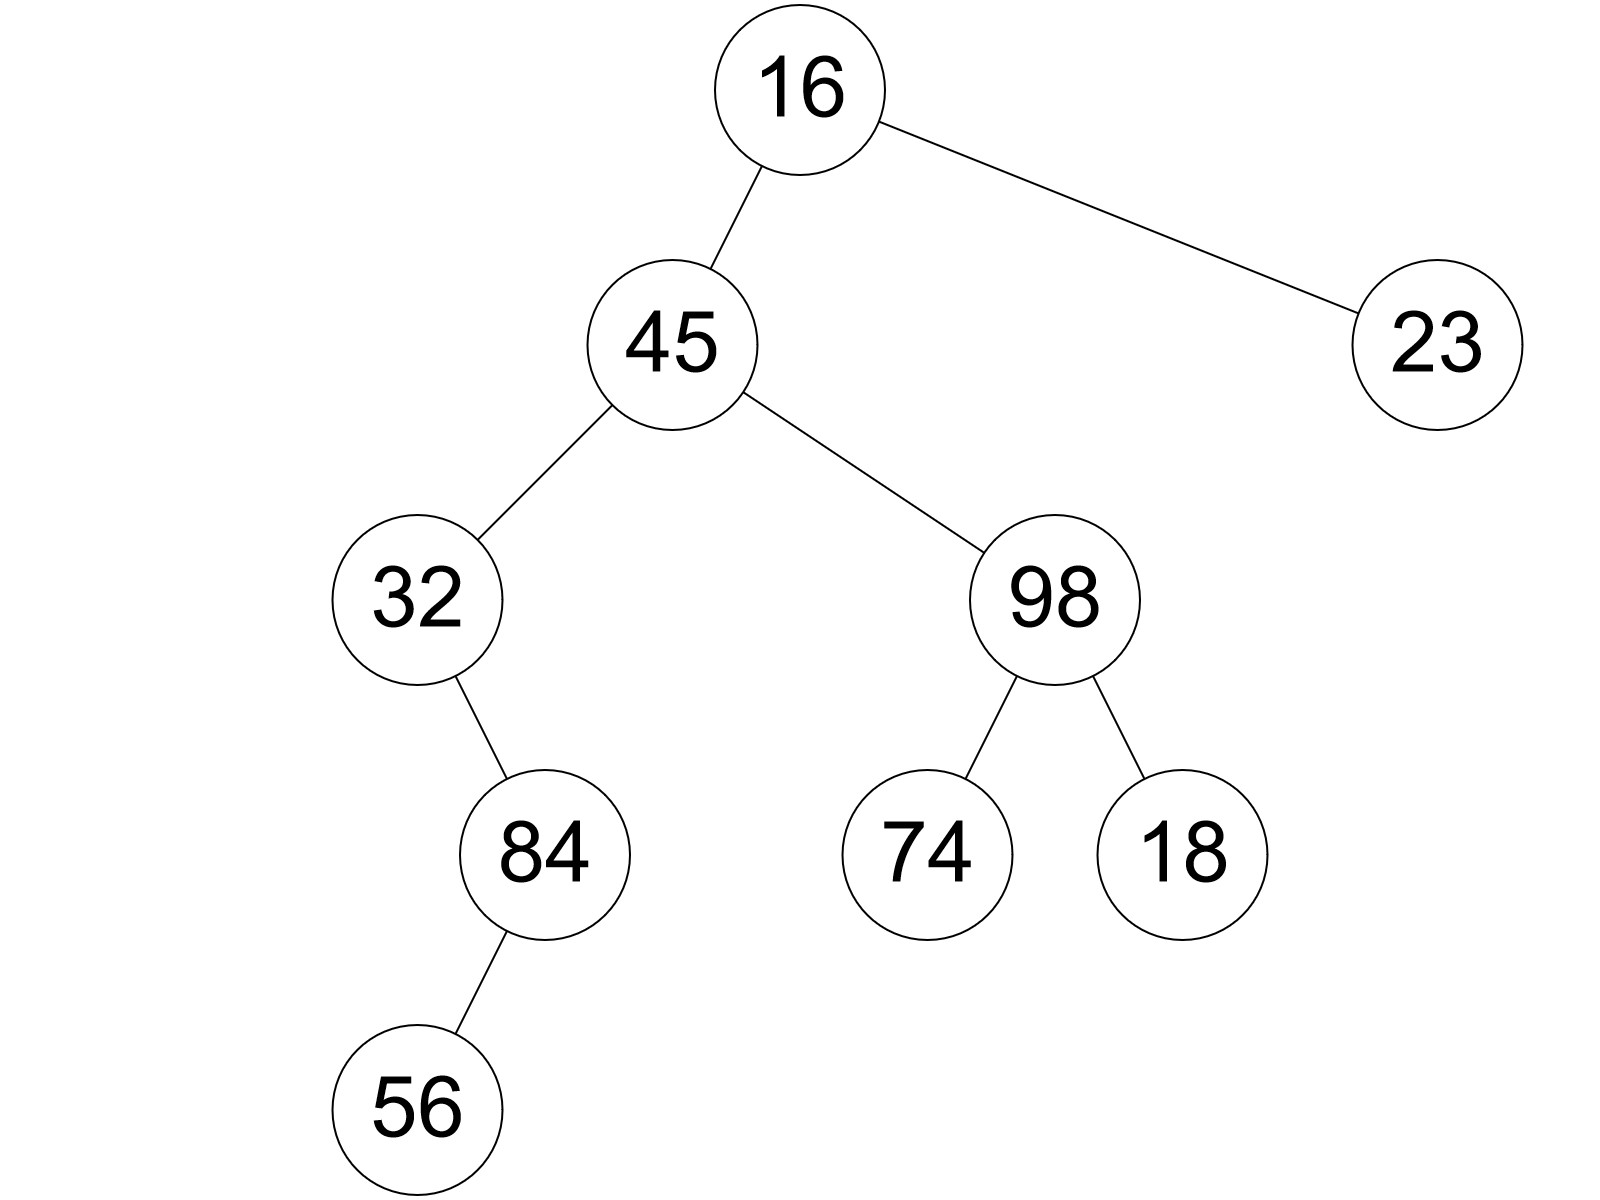
\includegraphics[width=0.4\textwidth]{img/4a_neu}
        \end{figure}
        \FloatBarrier
        \item Gegeben sei ein linksvoller, binärer, verketteter Baum mit Inorder-Darstellung (9, 8, 7, 6, 5, 4, 3, 2, 1).
        Wie sieht der Baum aus?
        \item Sei ein Knoten eines binären, verketteten Suchbaums durch folgende Datenstruktur definiert:
        \begin{lstlisting}[language=c++]
class Node {
    int value;
    Node *left, *right, *parent;
} 
        \end{lstlisting}
        Geben Sie einen Algorithmus in Pseudocode oder einer Programmiersprache Ihrer Wahl an, welcher Ihnen bei einem gegebenen Knoten den nächsten Knoten in Inorder-Reihenfolge liefert.
        \item
        Gegeben sei ein aufsteigend sortiertes Array mit $n$ ganzen Zahlen.
        Geben Sie einen Algorithmus mit Laufzeit $O(n)$ in Pseudocode oder einer Programmiersprache Ihrer Wahl an, welcher einen perfekt balancierten binär verketteten Suchbaum zurückgibt, der die gleichen Elemente wie das Array enthält.
    \end{enumerate}
\end{aufgabe}
\begin{loesung}
    \begin{enumerate}
        % \item \ \\
        % \begin{figure}[h!]
        %     \centering
        %     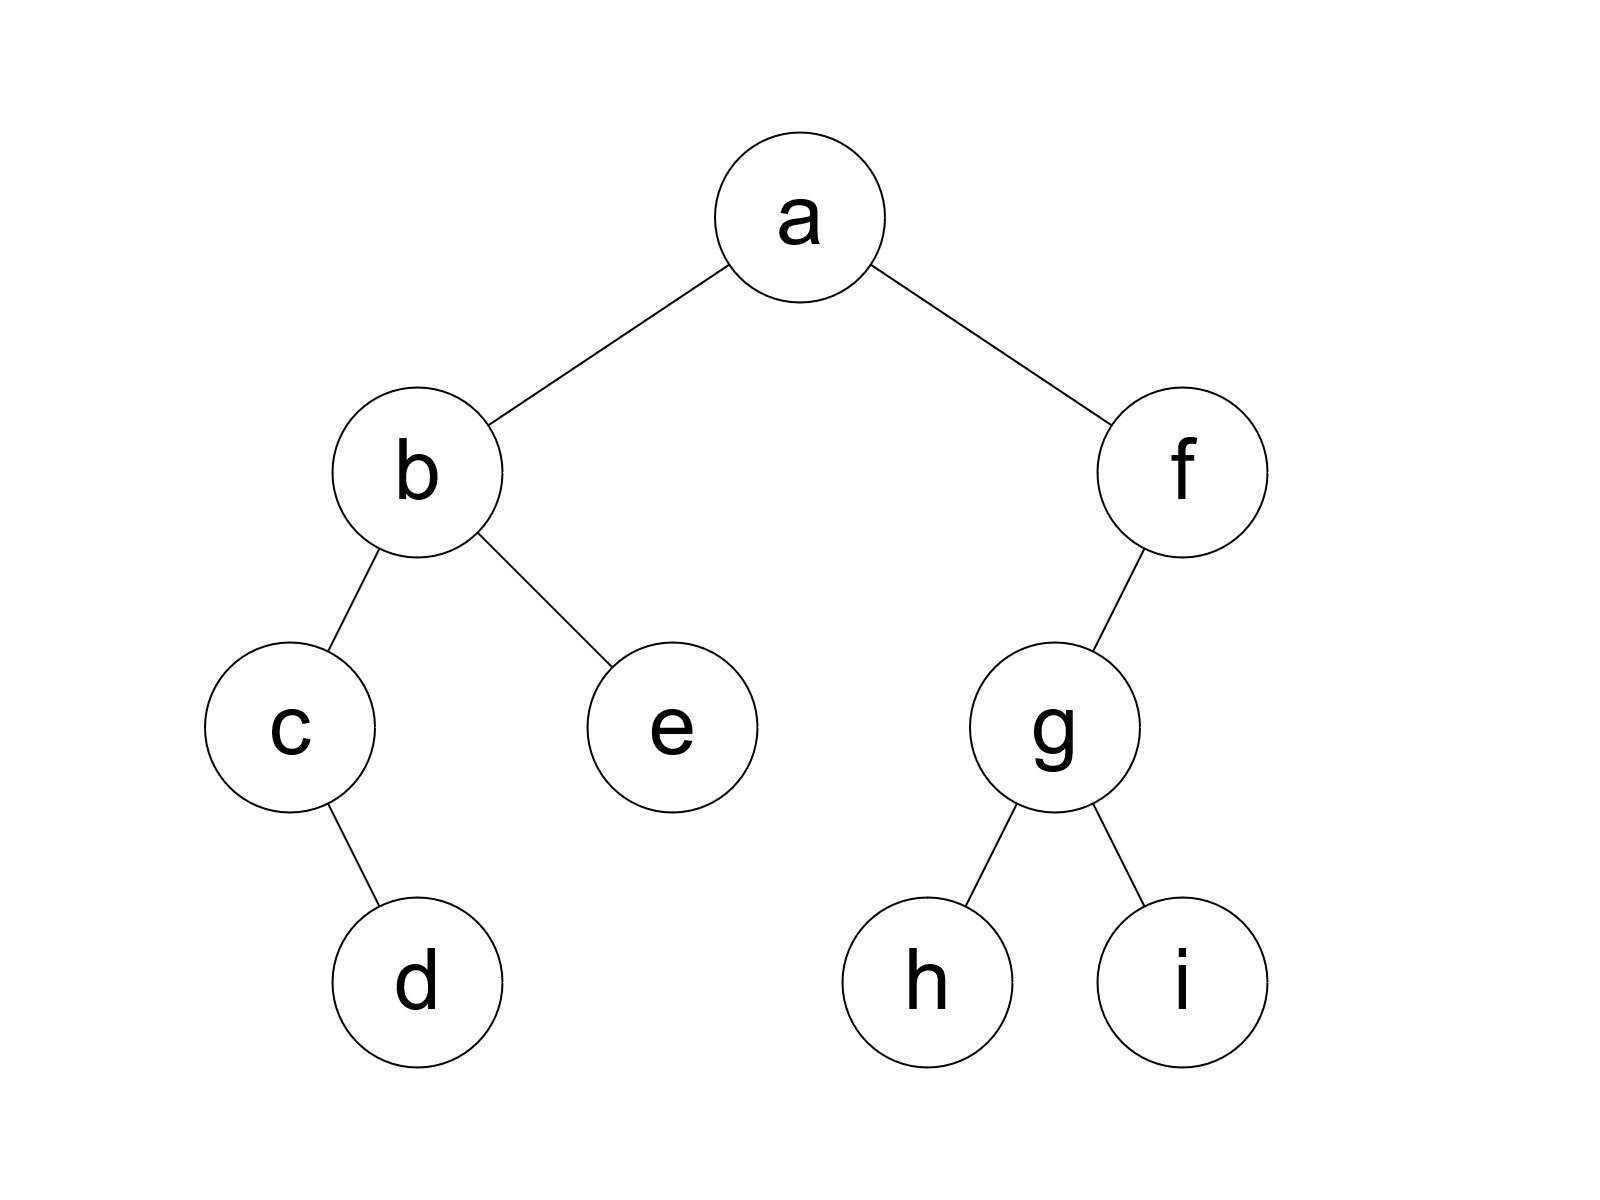
\includegraphics[width=0.3\textwidth]{img/4a}
        % \end{figure}
        % \FloatBarrier
        % \item \ \\
        % \begin{figure}[h!]
        %     \centering
        %     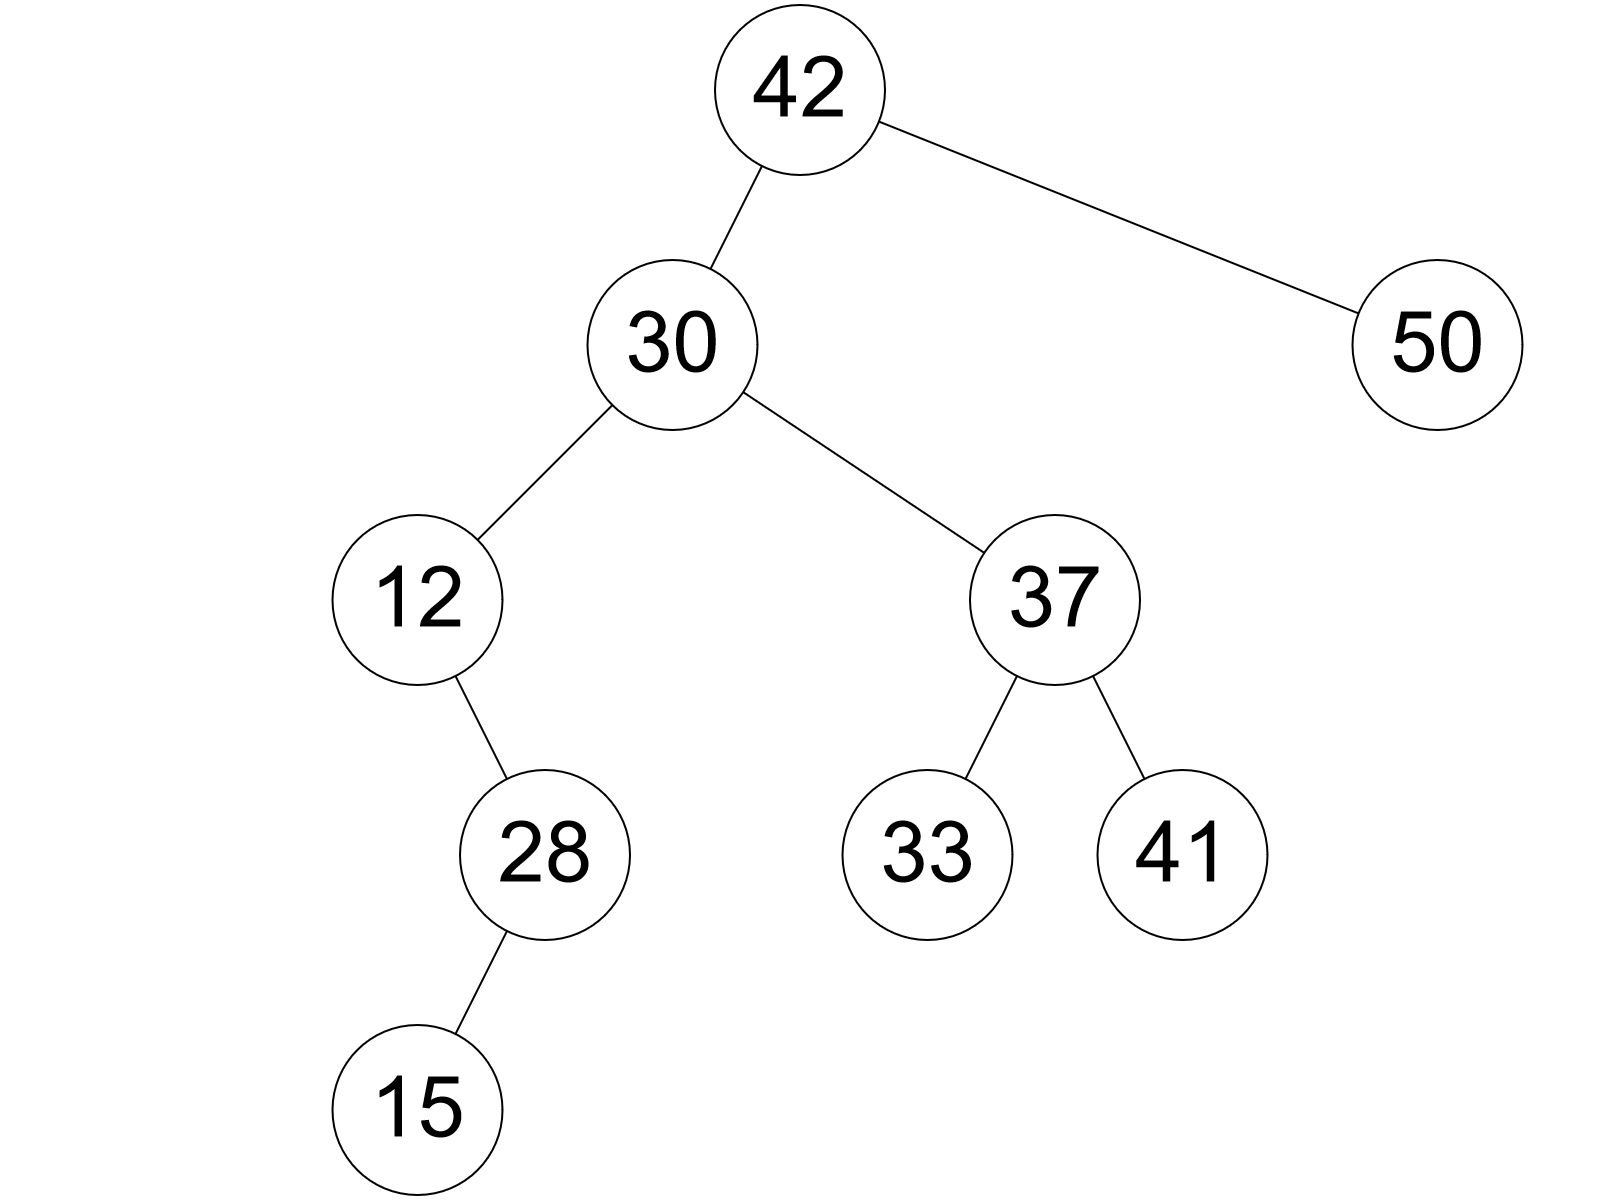
\includegraphics[width=0.3\textwidth]{img/4b}
        % \end{figure}
        % \FloatBarrier
        \item
        \begin{description}
            \item[Preorder] (16, 45, 32, 84, 56, 98, 74, 18, 23)
            \item[Inorder] (32, 56, 84, 45, 74, 98, 18, 16, 23)
            \item[Postorder] (56, 84, 32, 74, 18, 98, 45, 23, 16)
        \end{description}
        \item \ \\
        \begin{figure}[h!]
            \centering
            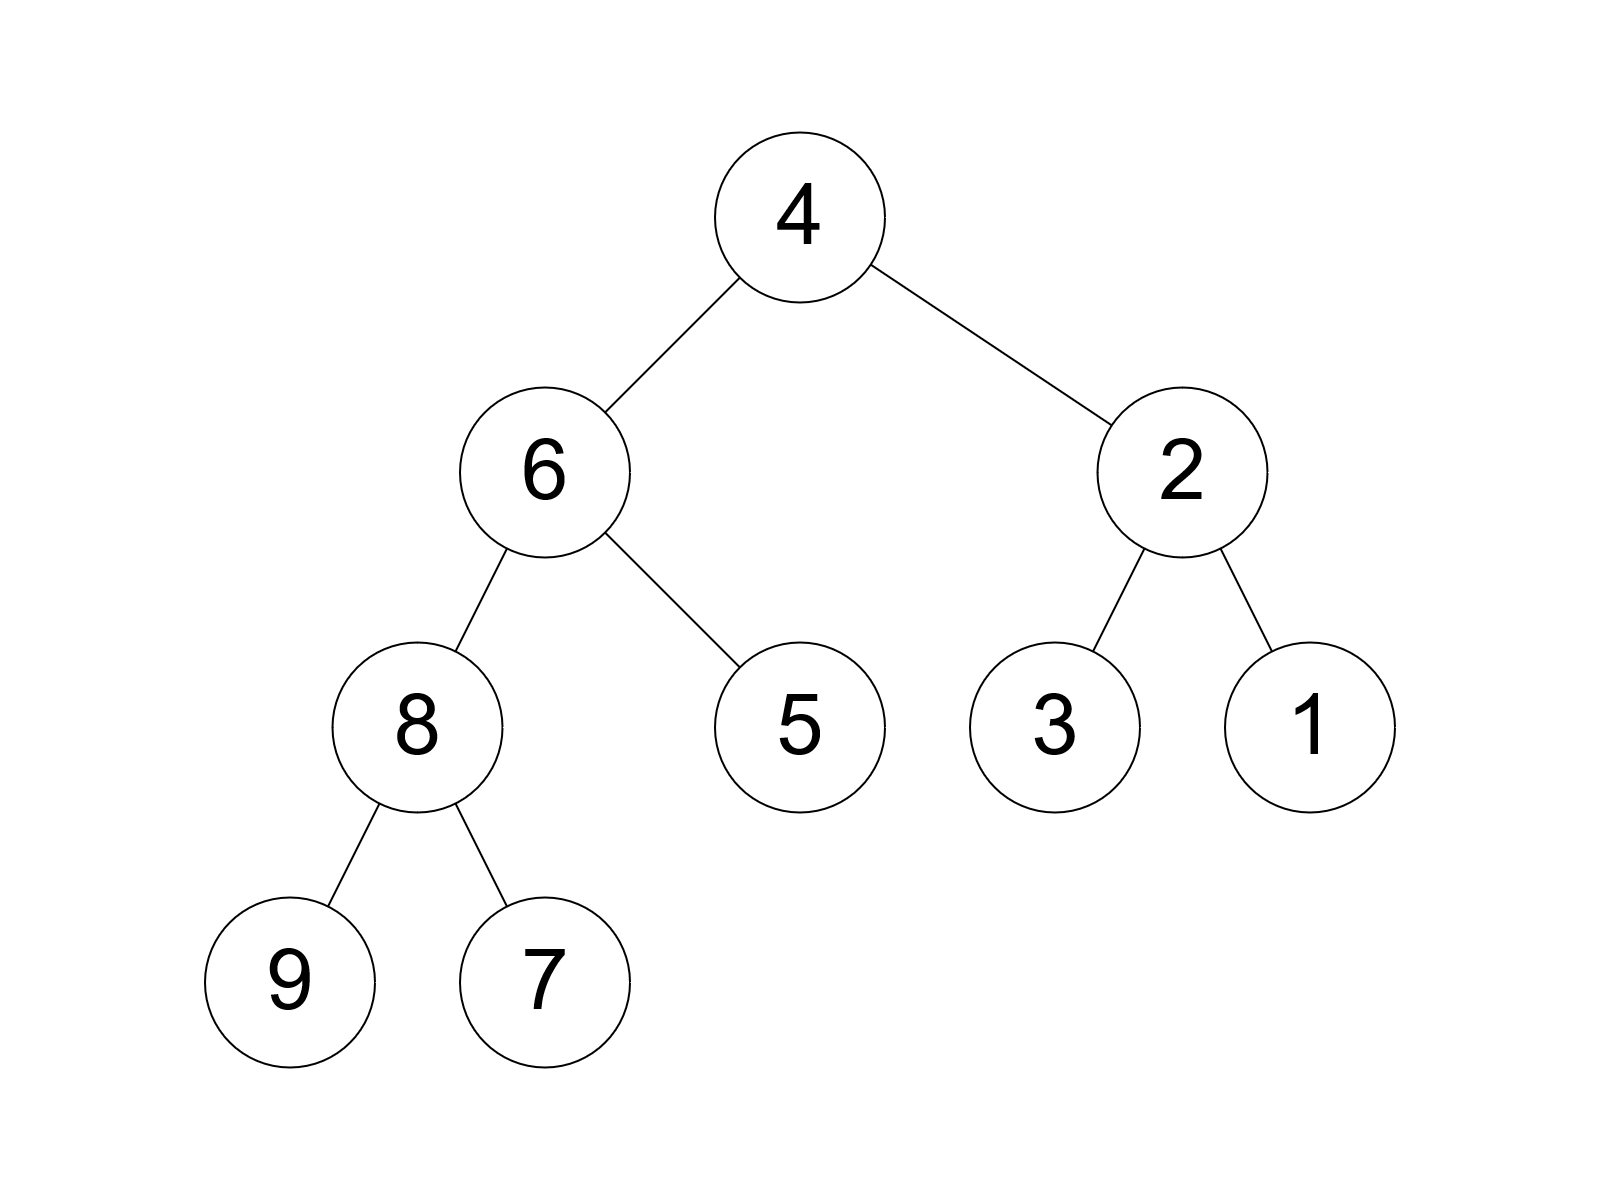
\includegraphics[width=0.3\textwidth]{img/4c}
        \end{figure}
        \FloatBarrier

        \item
        Wenn der Knoten einen rechten Nachfolger hat, dann ist der linkeste Knoten des Teilbaums unter dem rechten Nachfolger der nächste Knoten in Inorder-Reihenfolge.
        Falls der Knoten keinen rechten Nachfolger besitzt, liegt der nächste Knoten weiter oben im Baum.
        Bildlich muss man, um ihn zu finden, solange im Baum nach oben gehen, bis man einen Schritt nach rechts geht (in Inorder-Richtung).
        Dies passiert genau dann, wenn der vorherige Knoten auf dem Pfad zur Wurzel der linke Nachfolger des aktuellen betrachteten ist.
        Wird die Wurzel erreicht, bis man einen solchen Vorgängerknoten gefunden hat, gibt es keinen nächsten Knoten in Inorderreihenfolge.
        Der Knoten von dem aus die Suche gestartet wurde ist dann der letzte in Inorderreihenfolge.
        \begin{lstlisting}[language=c++]
Node *nextNode(Node *node) {
    if (node->right != nullptr) {
        // left-most node in right subtree
        Node *n = node->right;
        while (n->left != nullptr) {
            n = n->left;
        }
        return n;
    } else {
        // "right" parent (or grandparent or ...)
        Node *n = node;
        Node *p = node->parent;
        while (p != nullptr && n != p->left) {
            n = p;
            p = p->parent;
        }
        return p;
    }
}
        \end{lstlisting}

        \item 
        Damit der Baum balanciert ist, sollte der Wert in der Mitte des Arrays den Wurzelknoten bilden, sodass linker und rechter Teilbaum etwa gleich groß sind (wenn das Array eine gerade Anzahl an Elementen enthält, ist es aufgrund von Symmetrie egal, welchen der beiden mittleren Werten man wählt).
        Anschließend bilden die Elemente links neben dem gewählten Wurzelelement die Elemente des linken Teilbaums und die Elemente rechts danaben den rechten Teilbaum.
        Die beiden Teilbäume werden erstellt, indem der Algorithmus rekursiv aufgerufen wird.
        \begin{lstlisting}[language=c++]
Node *buildTree(int arr[], int start, int end, Node *parent) {
    if (end < start) {
        return nullptr;
    }
    int m = (start + end) / 2;
    Node *node = new Node;
    node->value = arr[m];
    node->left = buildTree(arr, start, m - 1, node);
    node->right = buildTree(arr, m + 1, end, node);
    node->parent = parent;
    return node;
}
Node *buildTree(int arr[], int n) {
    return buildTree(arr, 0, n - 1, nullptr);
}
        \end{lstlisting}
    \end{enumerate}
\end{loesung}


\end{document}